\documentclass[12pt]{beamer}
\usetheme{Berkeley}
\usepackage{graphicx}
\usepackage{booktabs}

\title{Jiskefet}

\author{Amin Chihab, Bastiaan Reinalda, Calvin Huynh, Misha Rigot, Ramon Gill}

\date{\today}

\begin{document}
	\begin{frame}
	\titlepage
	\end{frame}

	\begin{frame}{Overview}
		\tableofcontents
	\end{frame}

	% API
	
	\section{API}
	\begin{frame}
	    \frametitle{Application Programming Interface}
		endpoint: \texttt{api/logs}
   		
\includegraphics[scale=.40]{assets/logs.png}
		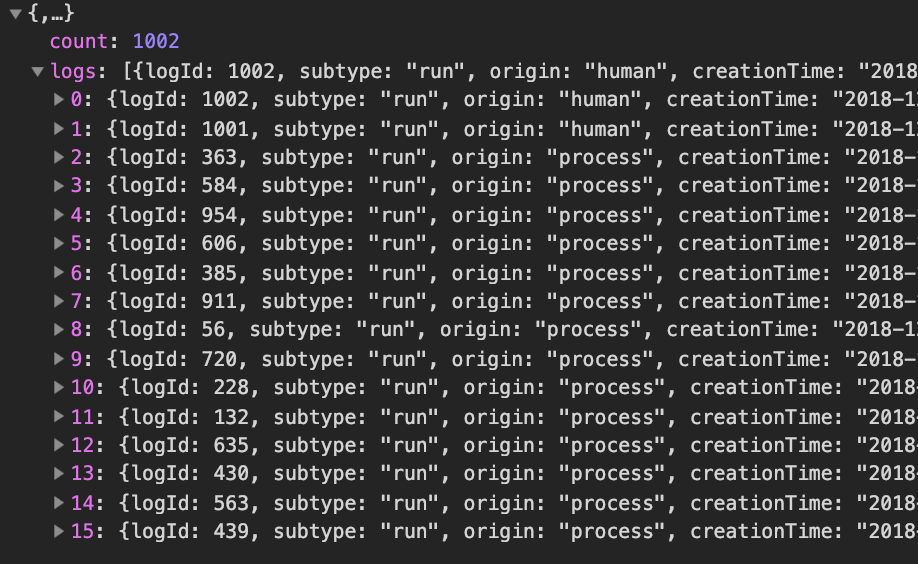
\includegraphics[scale=.45]{assets/logs_get_all_json.png}
    \end{frame}

	\begin{frame}
		\frametitle{Application Programming Interface}
		path: \texttt{src/controllers/log.controller.ts}
		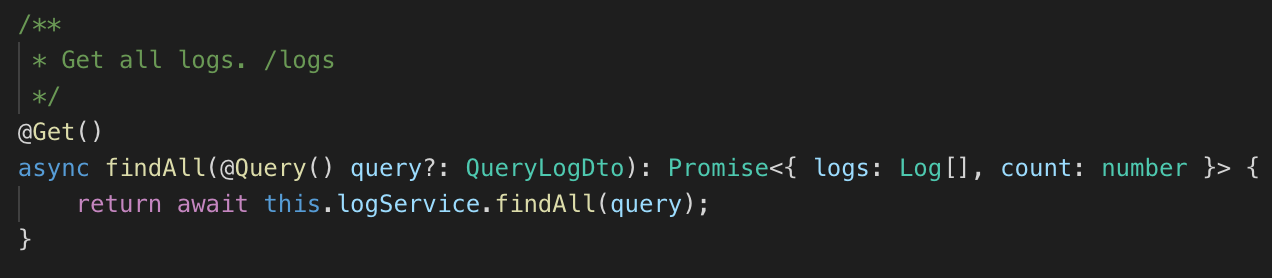
\includegraphics[scale=.45]{assets/logs_controller.png}
	\end{frame}

	\begin{frame}
		\frametitle{Application Programming Interface}
		path: \texttt{src/services/log.service.ts}
		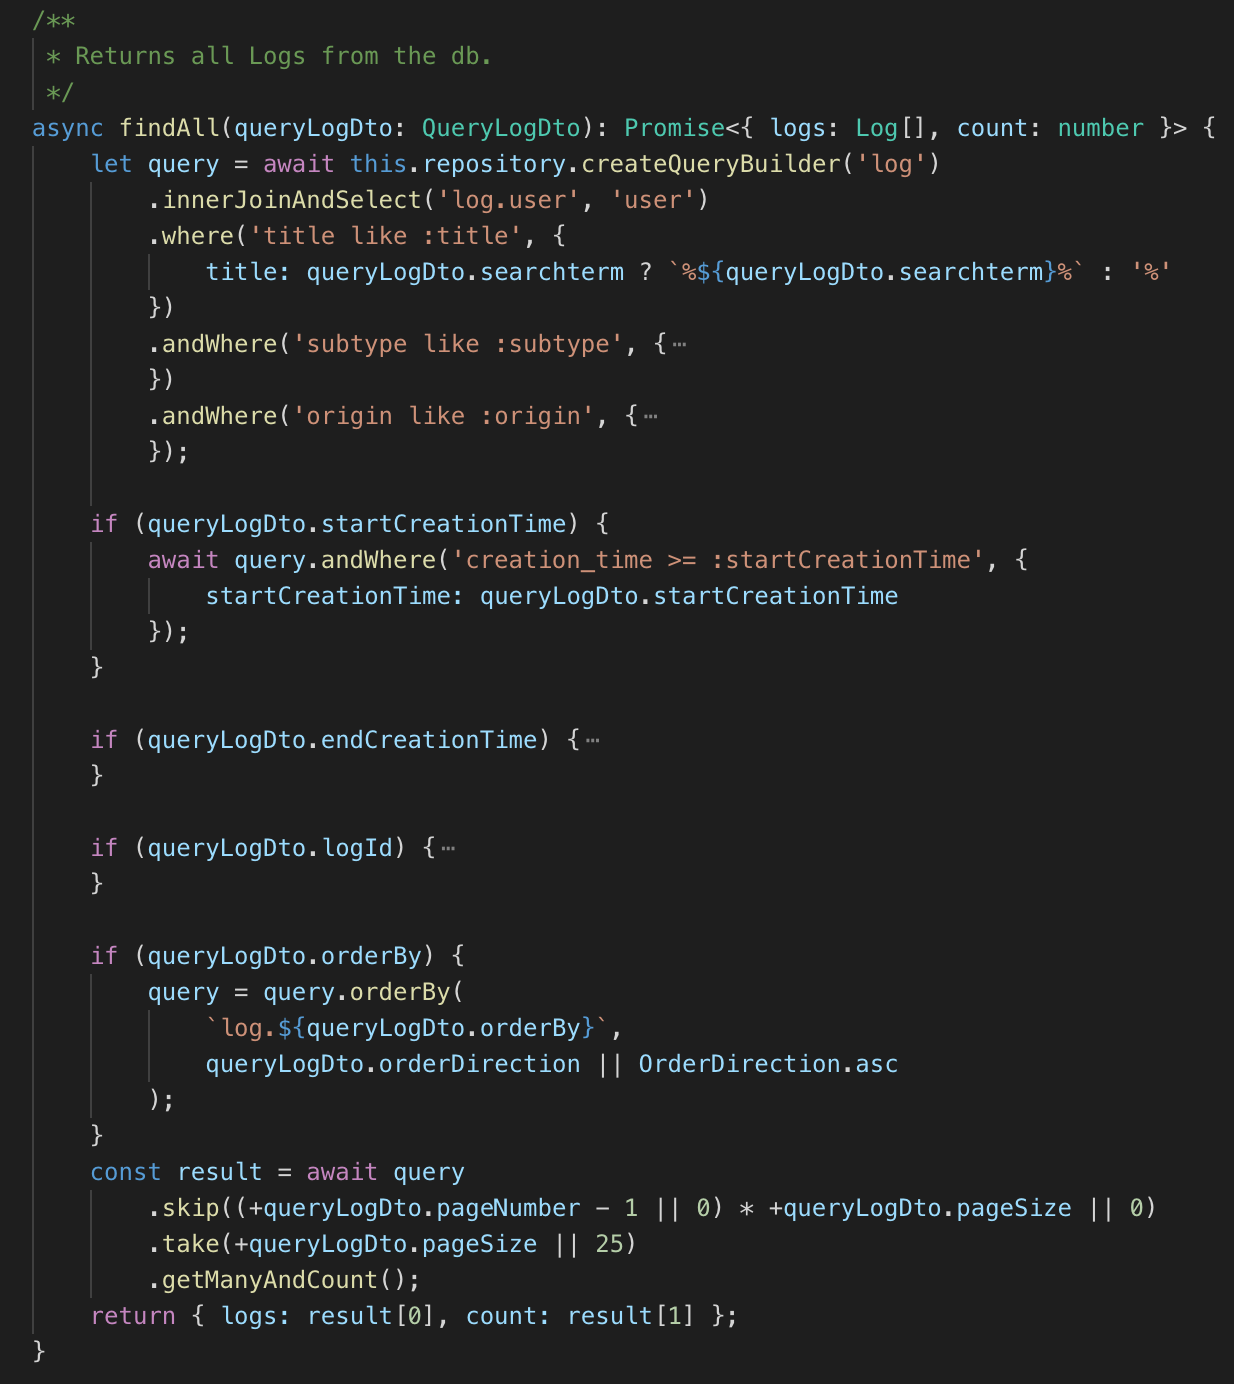
\includegraphics[scale=.3]{assets/logs_service.png}
	\end{frame}

    \begin{frame}
        \frametitle{Application Programming Interface}
        \begin{itemize}
        	\item Nest
        	\item Typeorm (MariaDB)
        	\item Jest
        	\item Structure
        \end{itemize}
    \end{frame}

	% UI
	\section{UI}
	\begin{frame}
		\frametitle{User Interface}
		\begin{itemize}
			\item Mithril
			\item Typescript
			\item Logs and Runs
			\item Markdown
			\item Authentication
			\item Token generation
		\end{itemize}
	\end{frame}

	% Documentation
	\section{Documentation}
	\begin{frame}
		\frametitle{Documentation}
		\begin{itemize}
			\item Markdown
			\item Instructions
		\end{itemize}
	\end{frame}

	% Performance
	\section{Performance}
	\begin{frame}
		\frametitle{Performance}
		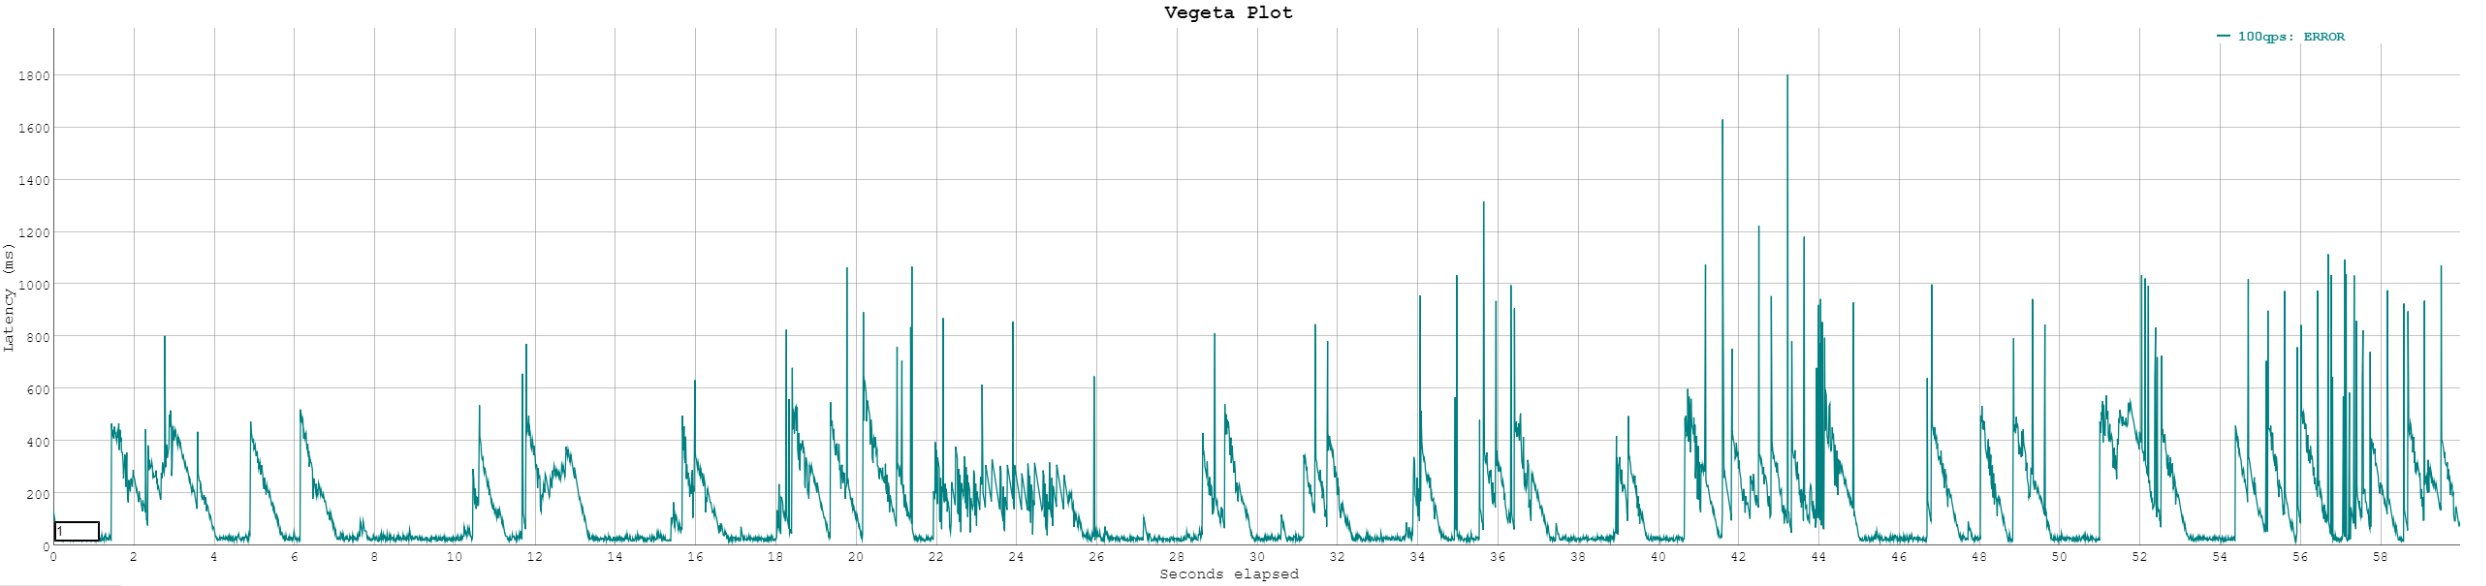
\includegraphics[scale=0.15]{assets/vegeta-plot.png}
		\begin{itemize}
			\item Benchmarks
			\item Vegeta
			\item Jest-Artillery
		\end{itemize}
	\end{frame}

	% Planning
	\section{Planning}
	\begin{frame}
		\frametitle{Planning}
		\begin{itemize}
			\item CERN SSO (logout)
			\item Front end testing
			\item Refactoring API
			\item Atomic Design
			\item Redux
			\item CI and more tests
		\end{itemize}
    \end{frame}
    


    % Deployment
	\section{Deployment}
	\begin{frame}
		\frametitle{Deployment}
		\begin{itemize}
			\item Ansible
			\begin{itemize}
                \item API
                \item UI
                \item Database
                \item Jenkins CI
            \end{itemize} 
			\item Jenkins CI
            \begin{itemize}
                \item Linting
                \item Testing
                \item Codecov
            \end{itemize}
		\end{itemize}
    \end{frame}

    \begin{frame}
        \frametitle{Deployment}
        jiskefet-deploy - Directory Structure Overview
        \newline
   		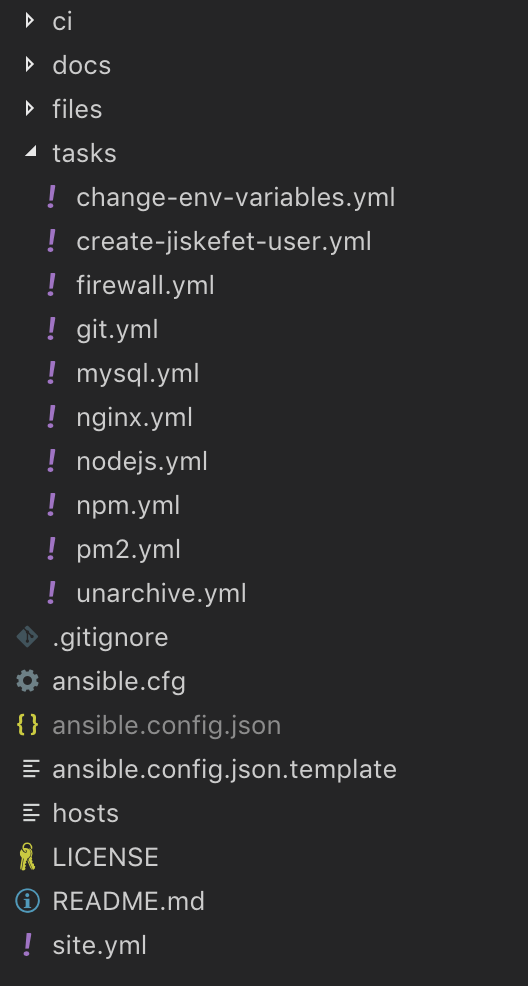
\includegraphics[scale=.40]{assets/deploy_dirstruct.png}
    \end{frame}

    \begin{frame}
        \frametitle{Deployment}
        Common tasks
        \newline
        path: \texttt{site.yml}
        \newline
   		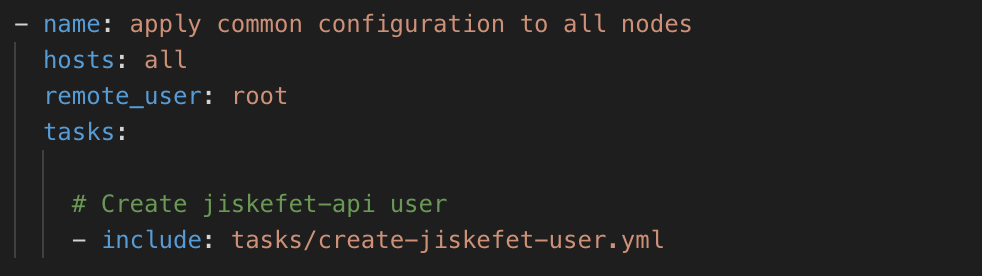
\includegraphics[scale=.40]{assets/deploy_create_user.png}
    \end{frame}
    
    \begin{frame}
        \frametitle{Deployment}
        Web server
        \newline
        path: \texttt{site.yml}
        \newline
   		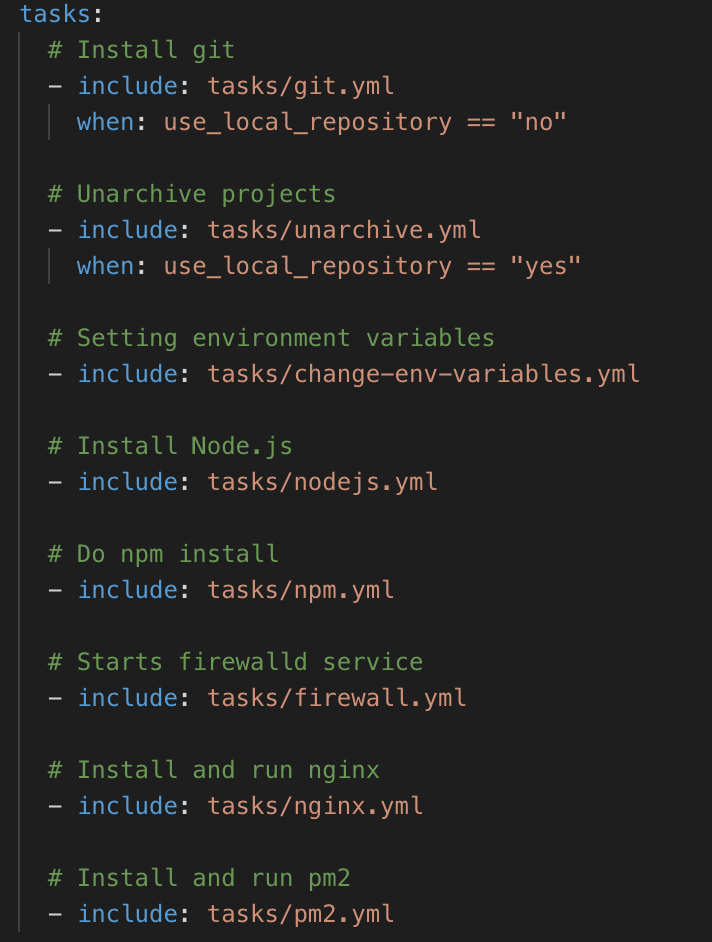
\includegraphics[scale=.30]{assets/deploy_webserver.png}
    \end{frame}
        
    \begin{frame}
        \frametitle{Deployment}
        Database server
        \newline
        path: \texttt{site.yml}
        \newline
   		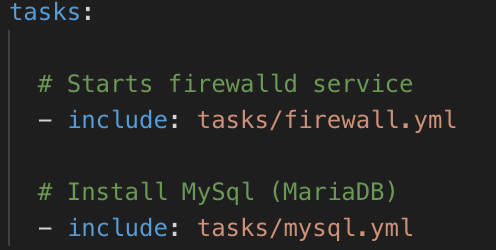
\includegraphics[scale=.30]{assets/deploy_databaseserver.png}
	\end{frame}
\end{document}